\begin{figure}[ht]
   \centering
   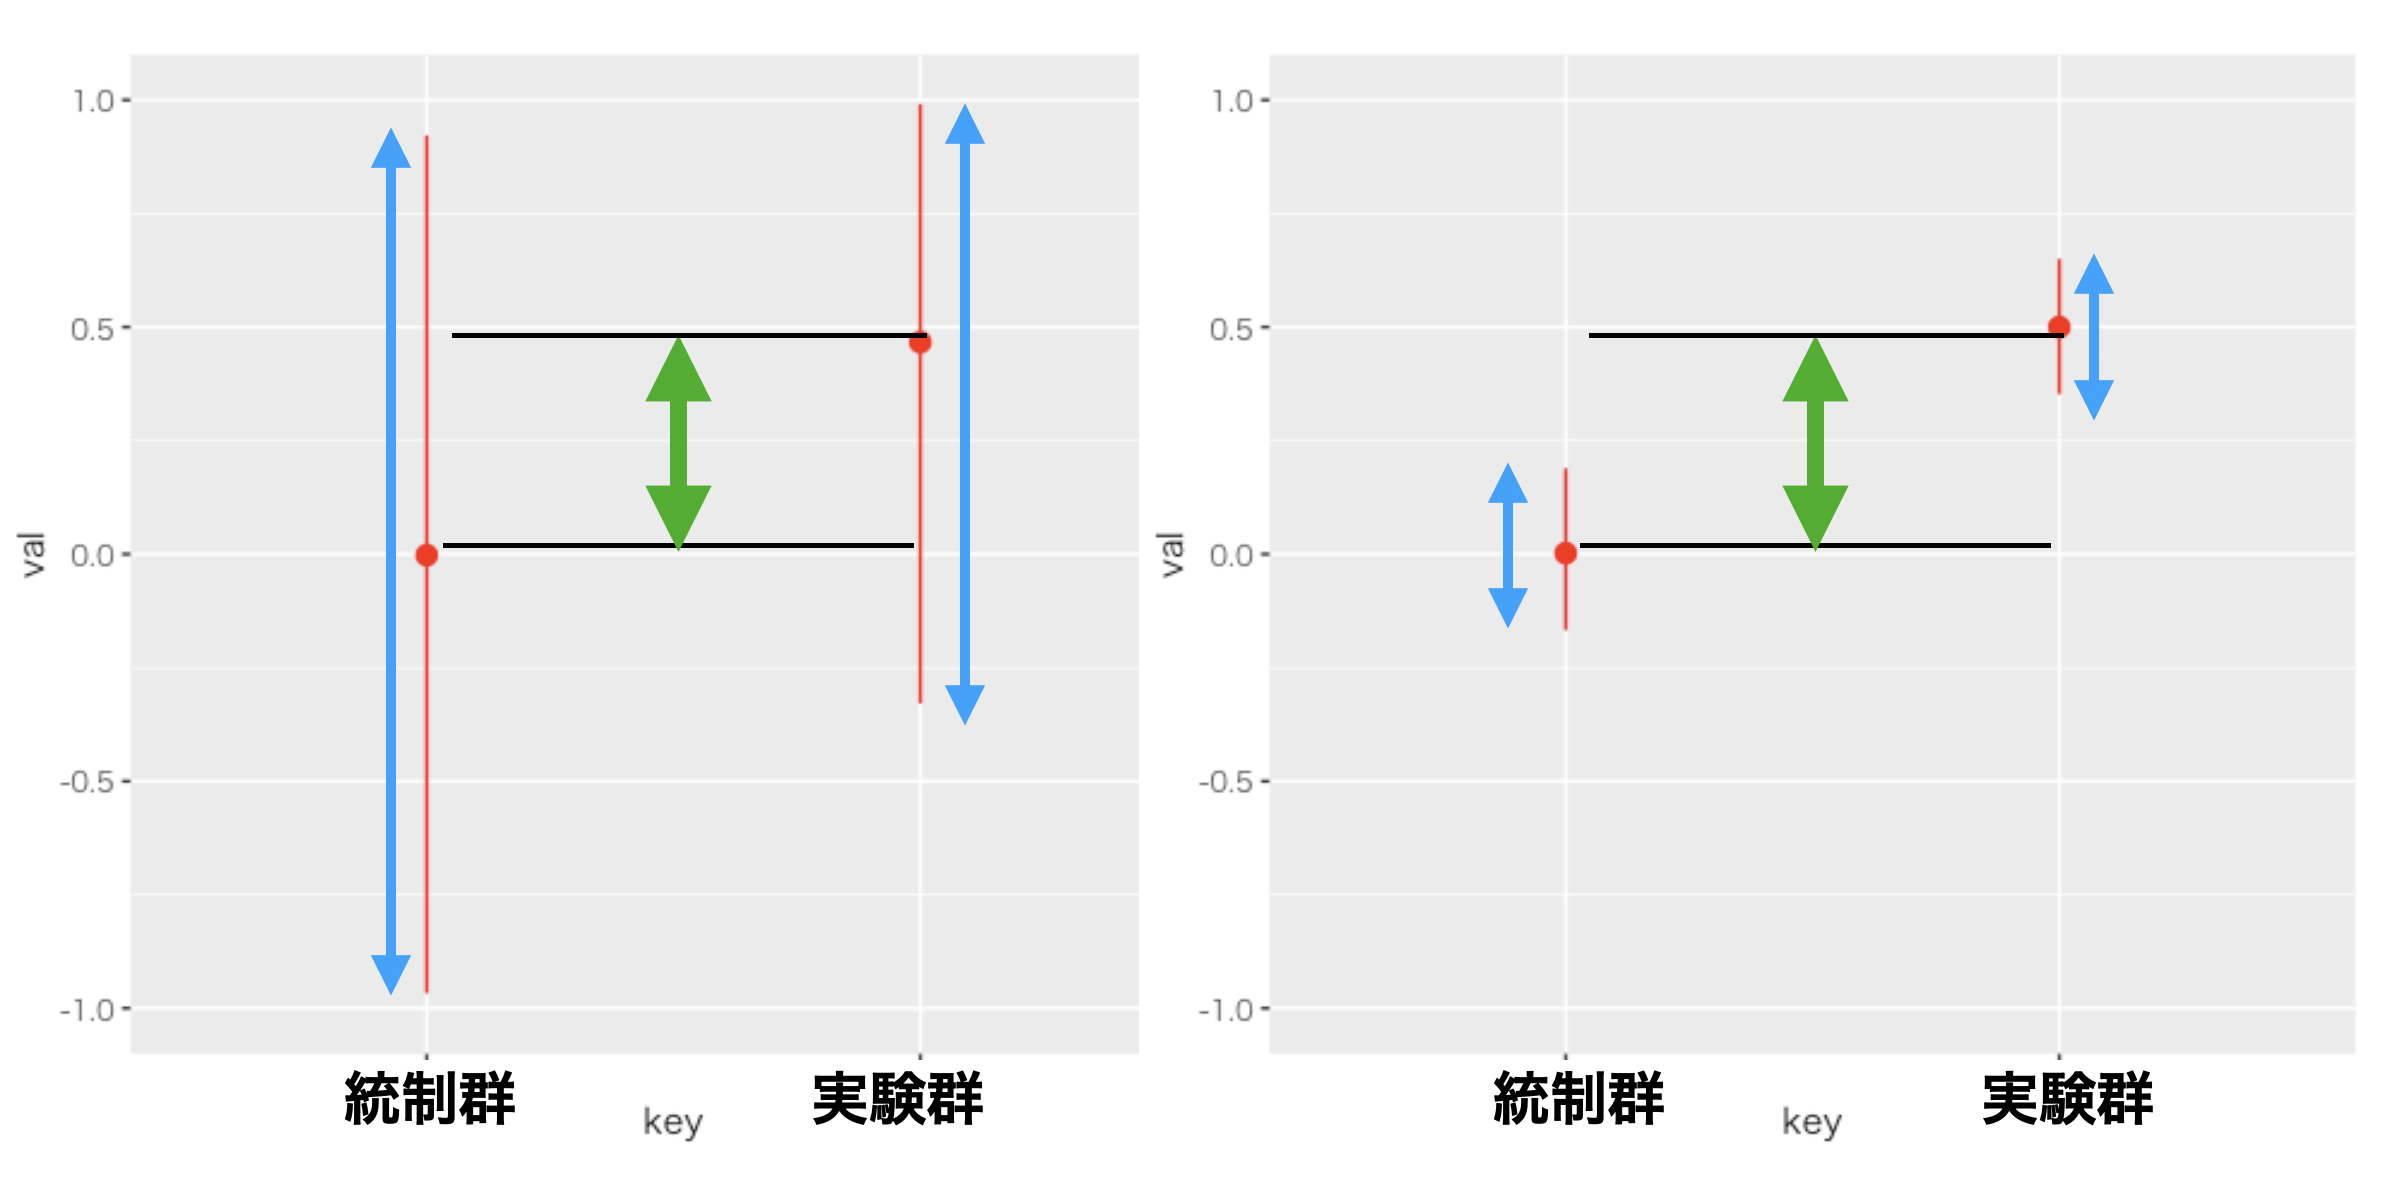
\includegraphics[keepaspectratio,width=0.8\linewidth]{../images/21_anova/slide21_08.png}
   \caption{Example of two experiments where the difference in mean (group effect) is the same. In the left example, it is difficult to say that there is an effect because the variation within groups (blue arrow) is greater than the variation between groups (green arrow). In the right example, it is easy to say that there is an effect since the maximum value in the control group is not even as high as the minimum value in the experimental group.}
   \label{fig::21_08}
\end{figure}
